\documentclass[12pt, spanish]{article}
\usepackage[spanish]{babel}
\selectlanguage{spanish}
%\usepackage{natbib}
\usepackage{url}
\usepackage[utf8x]{inputenc}
\usepackage{graphicx}
\graphicspath{{images/}}
\usepackage{parskip}
\usepackage{fancyhdr}
\usepackage{vmargin}
\usepackage{multirow}
\usepackage{float}
\usepackage{chngpage}

\usepackage{amsfonts}

\usepackage{subcaption}

\usepackage{hyperref}
\usepackage[
    type={CC},
    modifier={by-nc-sa},
    version={4.0},
]{doclicense}

\hypersetup{
    colorlinks=true,
    linkcolor=blue,
    filecolor=magenta,      
    urlcolor=cyan,
}

% para codigo
\usepackage{listings}
\usepackage{xcolor}



%% configuración de listings

\definecolor{listing-background}{HTML}{F7F7F7}
\definecolor{listing-rule}{HTML}{B3B2B3}
\definecolor{listing-numbers}{HTML}{B3B2B3}
\definecolor{listing-text-color}{HTML}{000000}
\definecolor{listing-keyword}{HTML}{435489}
\definecolor{listing-identifier}{HTML}{435489}
\definecolor{listing-string}{HTML}{00999A}
\definecolor{listing-comment}{HTML}{8E8E8E}
\definecolor{listing-javadoc-comment}{HTML}{006CA9}

\lstdefinestyle{eisvogel_listing_style}{
  language         = python,
%$if(listings-disable-line-numbers)$
%  xleftmargin      = 0.6em,
%  framexleftmargin = 0.4em,
%$else$
  numbers          = left,
  xleftmargin      = 0em,
 framexleftmargin = 0em,
%$endif$
  backgroundcolor  = \color{listing-background},
  basicstyle       = \color{listing-text-color}\small\ttfamily{}\linespread{1.15}, % print whole listing small
  breaklines       = true,
  frame            = single,
  framesep         = 0.19em,
  rulecolor        = \color{listing-rule},
  frameround       = ffff,
  tabsize          = 4,
  numberstyle      = \color{listing-numbers},
  aboveskip        = 1.0em,
  belowskip        = 0.1em,
  abovecaptionskip = 0em,
  belowcaptionskip = 1.0em,
  keywordstyle     = \color{listing-keyword}\bfseries,
  classoffset      = 0,
  sensitive        = true,
  identifierstyle  = \color{listing-identifier},
  commentstyle     = \color{listing-comment},
  morecomment      = [s][\color{listing-javadoc-comment}]{/**}{*/},
  stringstyle      = \color{listing-string},
  showstringspaces = false,
  escapeinside     = {/*@}{@*/}, % Allow LaTeX inside these special comments
  literate         =
  {á}{{\'a}}1 {é}{{\'e}}1 {í}{{\'i}}1 {ó}{{\'o}}1 {ú}{{\'u}}1
  {Á}{{\'A}}1 {É}{{\'E}}1 {Í}{{\'I}}1 {Ó}{{\'O}}1 {Ú}{{\'U}}1
  {à}{{\`a}}1 {è}{{\'e}}1 {ì}{{\`i}}1 {ò}{{\`o}}1 {ù}{{\`u}}1
  {À}{{\`A}}1 {È}{{\'E}}1 {Ì}{{\`I}}1 {Ò}{{\`O}}1 {Ù}{{\`U}}1
  {ä}{{\"a}}1 {ë}{{\"e}}1 {ï}{{\"i}}1 {ö}{{\"o}}1 {ü}{{\"u}}1
  {Ä}{{\"A}}1 {Ë}{{\"E}}1 {Ï}{{\"I}}1 {Ö}{{\"O}}1 {Ü}{{\"U}}1
  {â}{{\^a}}1 {ê}{{\^e}}1 {î}{{\^i}}1 {ô}{{\^o}}1 {û}{{\^u}}1
  {Â}{{\^A}}1 {Ê}{{\^E}}1 {Î}{{\^I}}1 {Ô}{{\^O}}1 {Û}{{\^U}}1
  {œ}{{\oe}}1 {Œ}{{\OE}}1 {æ}{{\ae}}1 {Æ}{{\AE}}1 {ß}{{\ss}}1
  {ç}{{\c c}}1 {Ç}{{\c C}}1 {ø}{{\o}}1 {å}{{\r a}}1 {Å}{{\r A}}1
  {€}{{\EUR}}1 {£}{{\pounds}}1 {«}{{\guillemotleft}}1
  {»}{{\guillemotright}}1 {ñ}{{\~n}}1 {Ñ}{{\~N}}1 {¿}{{?`}}1
  {…}{{\ldots}}1 {≥}{{>=}}1 {≤}{{<=}}1 {„}{{\glqq}}1 {“}{{\grqq}}1
  {”}{{''}}1
}
\lstset{style=eisvogel_listing_style}


\usepackage[default]{sourcesanspro}

\setmarginsrb{2 cm}{1 cm}{2 cm}{2 cm}{1 cm}{1.5 cm}{1 cm}{1.5 cm}

\title{Práctica 2:\\
Programación  \hspace{0.05cm} }                           
\author{Antonio David Villegas Yeguas}                             
\date{\today}                                           

\renewcommand*\contentsname{hola}

\makeatletter
\let\thetitle\@title
\let\theauthor\@author
\let\thedate\@date
\makeatother

\pagestyle{fancy}
\fancyhf{}
\rhead{\theauthor}
\lhead{\thetitle}
\cfoot{\thepage}

\begin{document}

%%%%%%%%%%%%%%%%%%%%%%%%%%%%%%%%%%%%%%%%%%%%%%%%%%%%%%%%%%%%%%%%%%%%%%%%%%%%%%%%%%%%%%%%%

\begin{titlepage}
    \centering
    \vspace*{0.3 cm}
    
\includegraphics[scale = 0.50]{ugr.png}\\[0.7 cm]
    %\textsc{\LARGE Universidad de Granada}\\[2.0 cm]   
    \textsc{\large 3º CSI 2019/20 - Grupo 1}\\[0.5 cm]            
    \textsc{\large Grado en Ingeniería Informática}\\[0.5 cm]              
    \rule{\linewidth}{0.2 mm} \\[0.2 cm]
    { \huge \bfseries \thetitle}\\
    \rule{\linewidth}{0.2 mm} \\[1 cm]
    
    \begin{minipage}{0.4\textwidth}
        \begin{flushleft} \large
            \emph{Autor:}\\
            \theauthor\\ 
			 \emph{DNI:}\\
            77021623-M
            \end{flushleft}
            \end{minipage}~
            \begin{minipage}{0.4\textwidth}
            \begin{flushright} \large
            \emph{Asignatura: \\
            AA}   \\     
            \emph{Correo:}\\
            advy99@correo.ugr.es           
        \end{flushright}
    \end{minipage}\\[0.5cm]
  
    {\large \thedate}\\[0.5cm]
    %{\url{https://github.com/advy99/AA/}}
    {\doclicenseThis}
 	
    \vfill
    
\end{titlepage}

%%%%%%%%%%%%%%%%%%%%%%%%%%%%%%%%%%%%%%%%%%%%%%%%%%%%%%%%%%%%%%%%%%%%%%%%%%%%%%%%%%%%%%%%%

\tableofcontents
\pagebreak

%%%%%%%%%%%%%%%%%%%%%%%%%%%%%%%%%%%%%%%%%%%%%%%%%%%%%%%%%%%%%%%%%%%%%%%%%%%%%%%%%%%%%%%%%

\section{Ejercicio sobre la complejidad de H y el ruido}

Este ejercicio consistirá en generar distintas nubes de puntos y clasificarlas según distintas funciones, en las que observaremos la dificultad que añade para la clasificación contar con ruido.

\subsection{Dibujo de la nube de puntos}

Para este apartado simplemente usaremos las funciones \texttt{simula\_unif} y \texttt{simula\_gauss} dadas:

\begin{lstlisting}

def simula_unif(N, dim, rango):
	return np.random.uniform(rango[0],rango[1],(N,dim))

def simula_gaus(N, dim, sigma):
    media = 0
    out = np.zeros((N,dim),np.float64)
    for i in range(N):
        # Para cada columna dim se emplea un sigma determinado. Es decir, para
        # la primera columna (eje X) se usará una N(0,sqrt(sigma[0]))
        # y para la segunda (eje Y) N(0,sqrt(sigma[1]))
        out[i,:] = np.random.normal(loc=media, scale=np.sqrt(sigma), size=dim)

    return out

\end{lstlisting}

\begin{figure}[H]
  \centering
      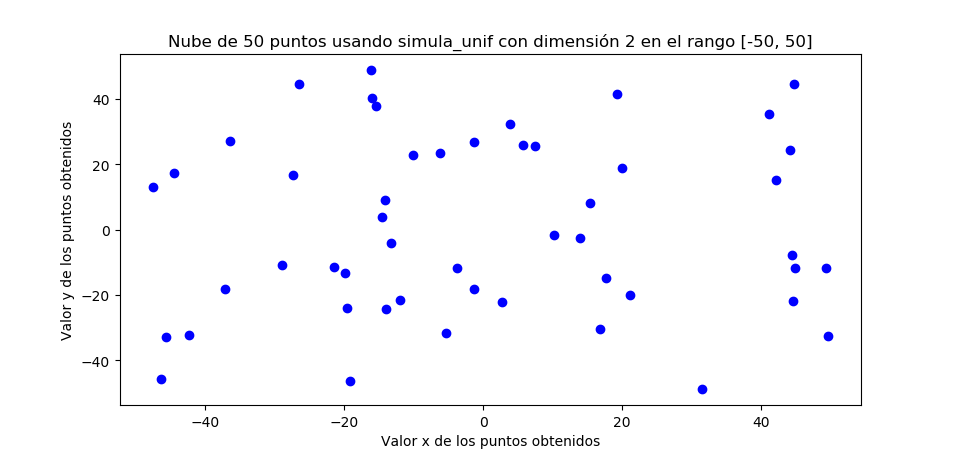
\includegraphics[scale = 0.70]{ej1-simula_unif.png}
 		 \caption{Puntos obtenidos usando simula\_unif}
  		\label{fig:ej1-1}

\end{figure}

\begin{figure}[H]
  \centering
      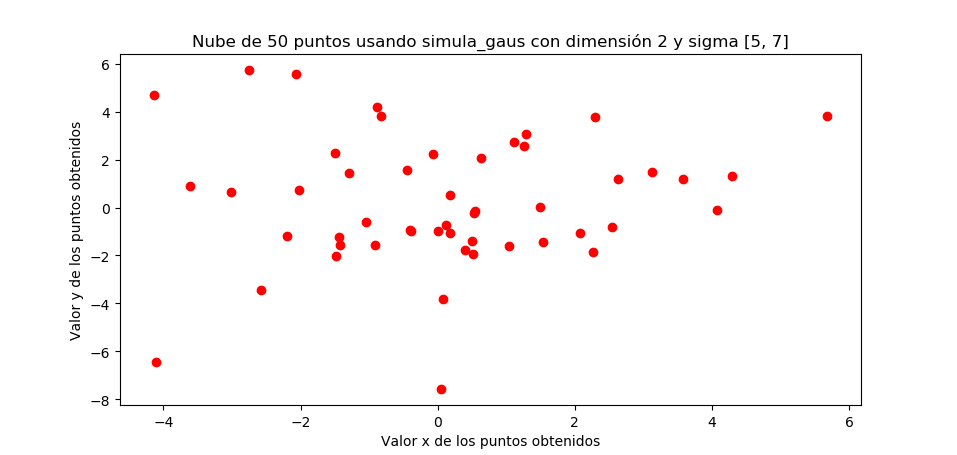
\includegraphics[scale = 0.70]{ej1-simula_gauss.png}
 		 \caption{Puntos obtenidos usando simula\_gauss}
  		\label{fig:ej1-2}

\end{figure}

Vemos como usando una distribución gaussiana, la mayor parte de los puntos están en el centro del intervalo, mientras que los sacados de forma uniforme se distribuyen de por todo el espacio.

Notar que el intervalo pedido para los puntos obtenidos de forma uniforme es [-50, 50] y los puntos obtenidos de forma gaussiana es de [5, 7]

\begin{figure}[H]
  \centering
      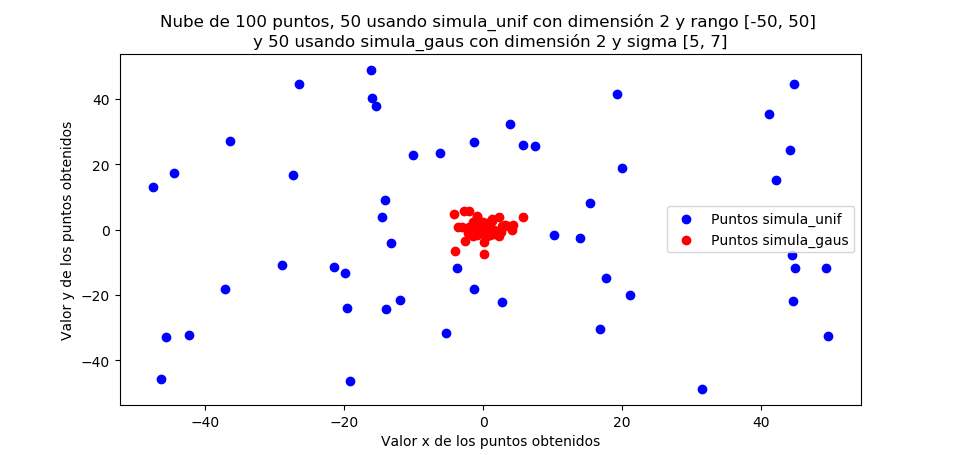
\includegraphics[scale = 0.70]{ej1_fin.png}
 		 \caption{Puntos obtenidos usando simula\_gauss y simula\_unif}
  		\label{fig:ej1-3}

\end{figure}


\subsection{Valoración del ruido}

En este ejercicio etiquetaremos 100 puntos obtenidos de forma uniforme en el intervalo [-50, 50] x [-50, 50] con una recta obtenida de forma aleatoria que pasa por ese intervalo. Una vez tenemos las etiquetas, aplicaremos un 10\% de ruido a las etiquetas evaluadas de forma positiva (a un lado de la recta) y otro 10\% de ruido a las etiquetas evaluadas de forma negativa (al otro lado de la recta), es decir, alteraremos un 10\% de las etiquetas de cada conjunto.

En el desarrollo del ejercicio veremos como es importante aplicar teniendo en cuenta las etiquetas originales, ya que si modificamos primero las positivas, y luego decidimos que negativas cambiar, podríamos estar cambiando una etiqueta de positiva a negativa, y nuevamente de negativa a positiva, por lo que la operación no tendría efecto.

\subsubsection{Etiquetado de los puntos usando una recta}

Para etiquetar los puntos, primero obtendremos una recta con la siguiente función:

\begin{lstlisting}
def simula_recta(intervalo):
    points = np.random.uniform(intervalo[0], intervalo[1], size=(2, 2))
    x1 = points[0,0]
    x2 = points[1,0]
    y1 = points[0,1]
    y2 = points[1,1]
    # y = a*x + b
    a = (y2-y1)/(x2-x1) # Calculo de la pendiente.
    b = y1 - a*x1       # Calculo del termino independiente.

    return a, b

\end{lstlisting}

Una vez obtenemos la recta, aplicaremos sobre los distintos puntos la siguiente función para comprobar si un punto está por encima o por debajo de dicha recta:

\begin{lstlisting}
# La funcion np.sign(0) da 0, lo que nos puede dar problemas
def signo(x):
	if x >= 0:
		return 1
	return -1

def f(x, y, a, b):
	return signo(y - a*x - b)

\end{lstlisting}

\newpage

De esta forma, obtendremos el etiquetado de todos los puntos, siendo el etiquetado binario, tomando los valores 1 o -1 como podemos ver en la función \texttt{signo}.


\begin{lstlisting}
intervalo_trabajo = [-50, 50]

puntos_2d = simula_unif(100, 2, intervalo_trabajo)

a, b = simula_recta(intervalo_trabajo)

etiquetas = []
posibles_etiquetas = (1, -1)
colores = {1: 'b', -1: 'r'}

for punto in puntos_2d:
	etiquetas.append(f(punto[0], punto[1], a, b))

\end{lstlisting}

Implementaremos también la siguiente función:

\begin{lstlisting}
def num_errores_puntos_f(x, y):

	errores = 0
	for i in range(len(x)):
		if signo(f(x[i])) != y[i]:
			errores += 1

	errores = errores/len(x)

	return errores
\end{lstlisting}

Que como vemos, nos dará el porcentaje de puntos mal clasificados usando la misma función f con la que hemos clasificado.


Tras esto, podemos dibujar los puntos y dicha recta, dando el siguiente resultado:

\begin{figure}[H]
  \centering
      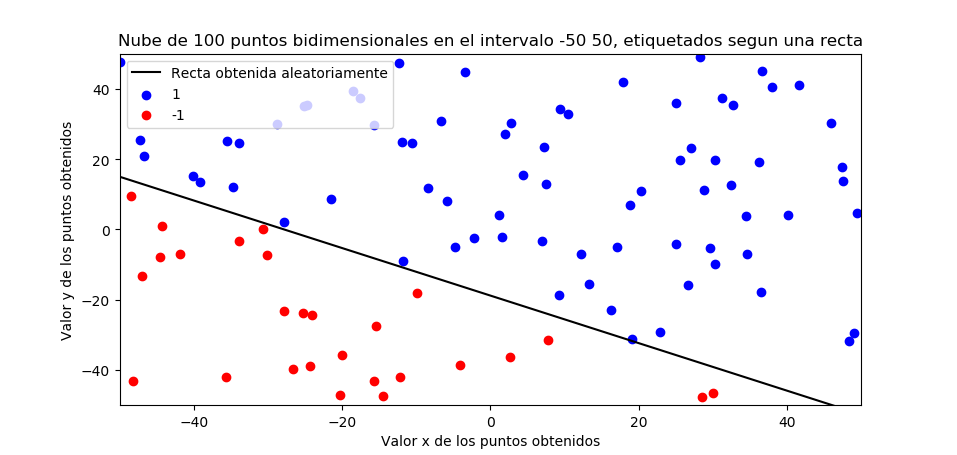
\includegraphics[scale = 0.70]{ej1-2-1.png}
 		 \caption{Puntos obtenidos usando simula\_unif etiquetados según la recta}
  		\label{fig:ej1-2-1}

\end{figure}


Vemos como en este caso, no existen puntos mal etiquetados, como cabía esperar:

\begin{lstlisting}
Porcentaje de errores en el etiquetado:  0.0
\end{lstlisting}

\newpage

\subsubsection{Aplicación del ruido a los datos}

Tras obtener esta recta, procedemos a aplicar el ruido al 10\% de cada etiqueta, como vemos en el siguiente código:

\begin{lstlisting}
# no podemos usar el for, tenemos que sacarlos a la vez
# si hacemos primero unos, al meter el ruido en el positivo, pasan a ser negativo,
# y se les podría llegar a meter ruido otra vez al hacer el ruido del negativo
indices_positivos = np.where(np.array(etiquetas) == 1)
indices_positivos = indices_positivos[0]

indices_negativos = np.where(np.array(etiquetas) == -1)
indices_negativos = indices_negativos[0]


# aplicamos el ruido a los positivos
num_a_aplicar = len(indices_positivos) * 0.1
num_a_aplicar = int(round(num_a_aplicar))
indices = np.random.choice(indices_positivos, num_a_aplicar, replace=False)

for i in indices:
	etiquetas[i] = -etiquetas[i]

# aplicamos el ruido a los negativos
num_a_aplicar = len(indices_negativos) * 0.1
num_a_aplicar = int(round(num_a_aplicar))
indices = np.random.choice(indices_negativos, num_a_aplicar, replace=False)

for i in indices:
	etiquetas[i] = -etiquetas[i]

\end{lstlisting}

Como antes comentamos, primero tenemos que obtener los indices, y después aplicar el ruido, si aplicamos el ruido en uno de los indices, y despues obtenemos los indices para aplicar el otro, el segundo conjunto se verá afectado por las etiquetas del primero a las que se les ha aplicado el ruido. El resultado final es el siguiente:


\begin{figure}[H]
  \centering
      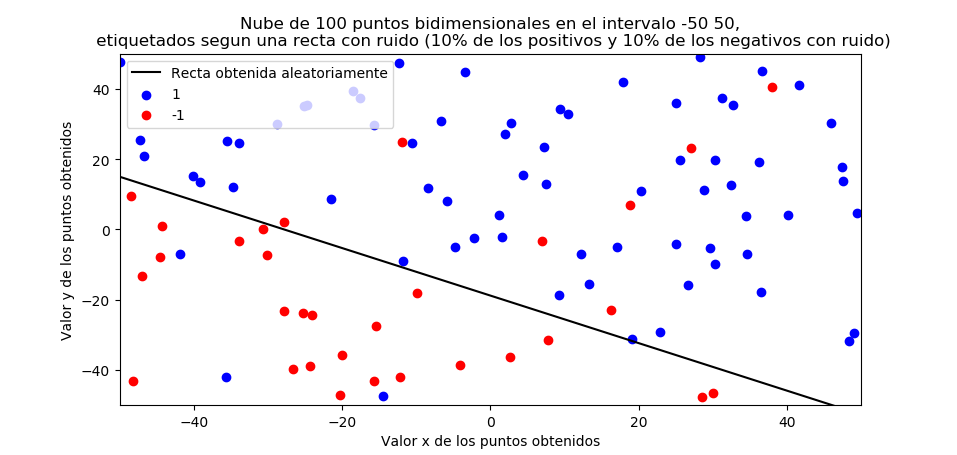
\includegraphics[scale = 0.70]{ej-1-2-2-ruido.png}
 		 \caption{Función $E(u,v)$}
  		\label{fig:ej1-2}

\end{figure}

En este caso, como cabía esperar, tenemos un 10\% de puntos mal clasificados debido al ruido introducido.

\begin{lstlisting}
Porcentaje de errores en el etiquetado:  0.1
\end{lstlisting}



\subsubsection{Uso de distintas funciones para definir la frontera y conclusiones}

En este apartado debemos cambiar la función con la que dibujamos la frontera de clasificación, es decir vamos a intentar clasificar los puntos con ruido usando distintas funciones.

En este caso, hemos modificado la función para comprobar el número de puntos mal clasificados para que se adapte a las funciones usadas:

\begin{lstlisting}
def num_errores_puntos_f_n(fun, x, y):

	errores = 0
	val = fun(x)
	for i in range(len(x)):
		if signo(val[i]) != y[i]:
			errores += 1

	errores = errores/len(x)

	return errores
\end{lstlisting}

\textbf{Función 1:} 

$$ f(x, y)_1 = (x - 10)^2 + (y - 20)^2 - 400  $$

\begin{figure}[H]
  \centering
      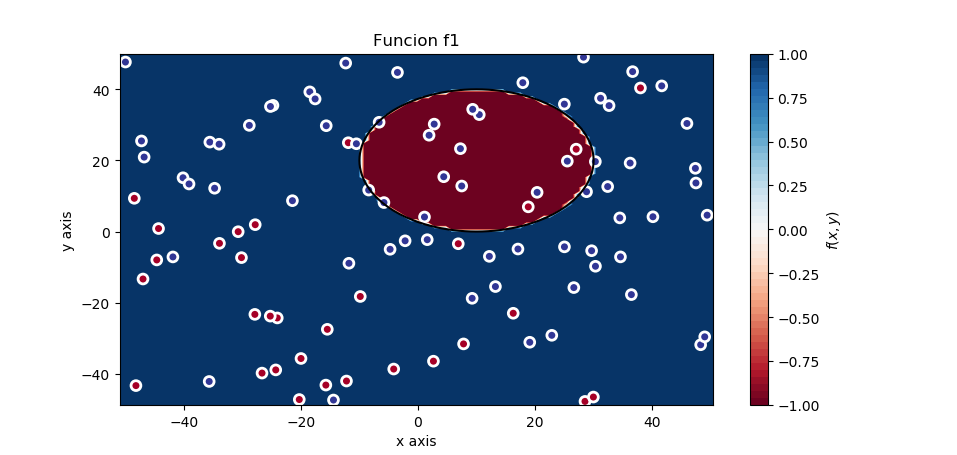
\includegraphics[scale = 0.70]{ej1-3-f1.png}
 		 \caption{Función $f(x, y)_1$}
  		\label{fig:ej1-f1}

\end{figure}

\begin{lstlisting}
Porcentaje de errores en el etiquetado usando f1:  0.41
\end{lstlisting}

Vemos como en este caso el ajuste es muy malo, ya que estamos visualizando unos puntos etiquetados con una recta aleatoria a los que hemos aplicado ruido con una función arbitraria. Esto sumado al ruido, hace que sea muy difícil obtener un buen clasificador.

\textbf{Función 2:} 

$$ f(x, y)_2 = 0,5*(x + 10)^2 + (y - 20)^2 - 400  $$

\begin{figure}[H]
  \centering
      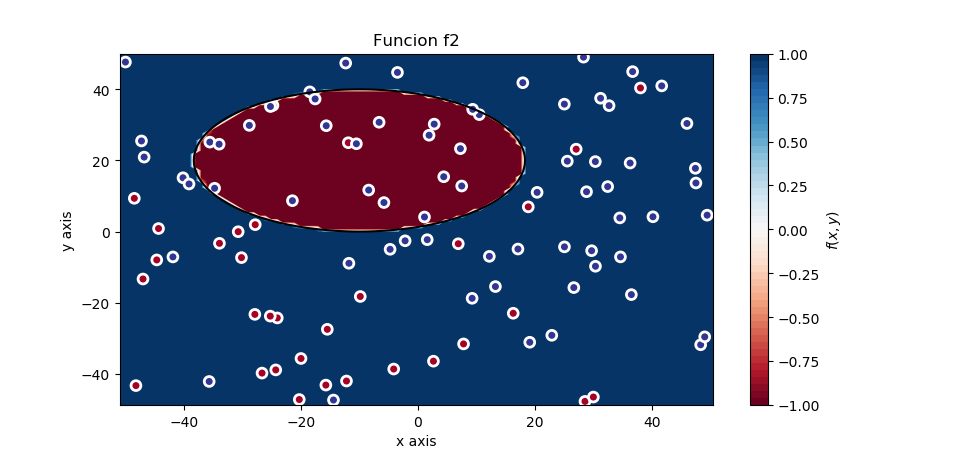
\includegraphics[scale = 0.70]{ej1-3-f2.png}
 		 \caption{Función $f(x, y)_2$}
  		\label{fig:ej1-f2}

\end{figure}

\begin{lstlisting}
Porcentaje de errores en el etiquetado usando f2:  0.51
\end{lstlisting}

De nuevo esto se repite con la segunda función por los mismos motivos que he comentado en la primera función.


\textbf{Función 3:} 

$$ f(x, y)_3 = 0,5*(x - 10)^2 + (y + 20)^2 - 400 $$

\begin{figure}[H]
  \centering
      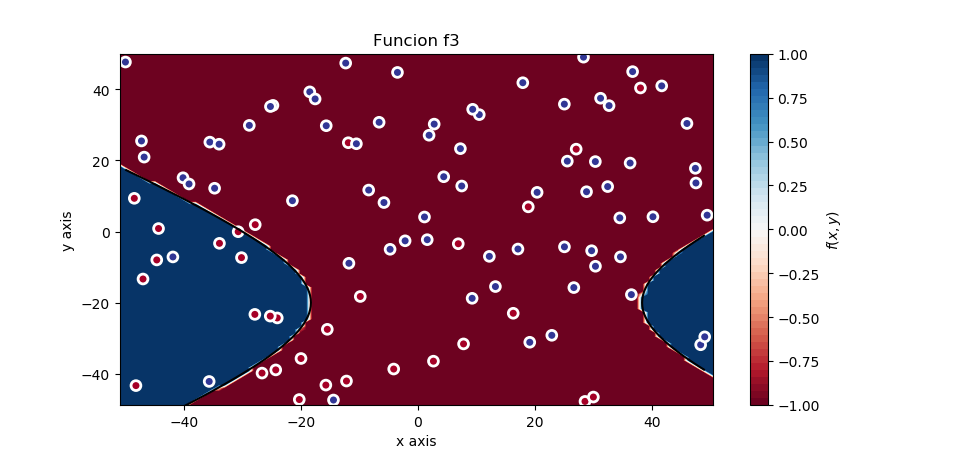
\includegraphics[scale = 0.70]{ej1-3-f3.png}
 		 \caption{Función $f(x, y)_3$}
  		\label{fig:ej1-f3}

\end{figure}

\begin{lstlisting}
Porcentaje de errores en el etiquetado usando f3:  0.76
\end{lstlisting}


\textbf{Función 4:} 

$$ f(x, y)_4 = y - 20*x^2 -5*x +3  $$

\begin{figure}[H]
  \centering
      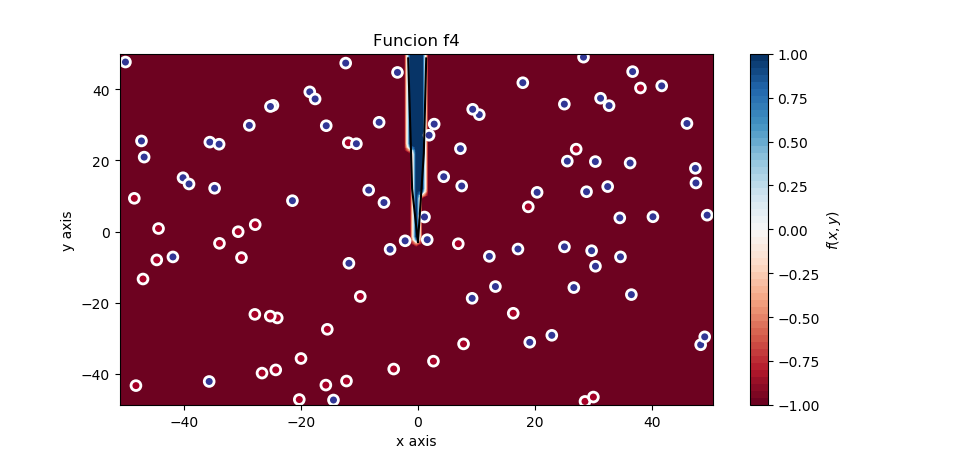
\includegraphics[scale = 0.70]{ej1-3-f4.png}
 		 \caption{Función $f(x, y)_4$}
  		\label{fig:ej1-f4}

\end{figure}

\begin{lstlisting}
Porcentaje de errores en el etiquetado usando f4:  0.69
\end{lstlisting}


Vemos como lo que comente para la primera función se sigue repitiendo con todas, y es que el que una función sea más compleja no implica mejores clasificadores, ya que las etiquetas se han obtenido con una función lineal. En este sentido, la calidad de un clasificador dependerá de con que se han etiquetado los valores, y el ruido aplicado, por ejemplo, si solo aplicamos ruido a las etiquetas cuya distancia de la recta es menor que un $\delta$, o incluso sin aplicar ruido,  la clasificación con otras funciones más complejas nos daría resultados mucho mejores si conseguimos que esas funciones complejas contengan la mayor parte del espacio sin pasar al otro lado de la recta.

De hecho vemos como llegamos a porcentajes enormes en los errores al etiquetar, ya que al usar clases más complejas no se adaptan de ninguna forma, y puede ocurrir como en el caso 4, en los que al no etiquetar ningún punto en la zona azul, el error es más bajo que en la función 3 ya que todos los rojos si que los etiqueta de forma correcta.

Como conclusión, no solo en este ejercicio sino en general, el ruido hace que sea mucho más complejo obtener un buen clasificador debido a que la frontera es mucho más grande e incluso, como en este ejemplo, es posible que amplíe la frontera a todo el espacio en el que trabajamos, al poder aplicar el ruido a cualquier etiqueta. Si aplicamos el ruido exclusivamente a etiquetas cercanas a la función con la que etiquetamos, seguimos manteniendo la frontera, aunque un poco mayor.

\newpage

\section{Modelos lineales}

En este ejercicio implementaremos dos métodos lineales, el algoritmo Perceptron y Regresión Logística con Gradiente Descendente Estocástico para estudiar como se comportan estos algoritmos.

\subsection{Algoritmo Perceptron}

\subsubsection{Implementación del algoritmo}

El algoritmo Perceptron se basa en actualizar el vector de pesos w dependiendo del signo de los datos, de forma que el vector de pesos se vaya modificando hasta que tenga todos los datos correctamente clasificados, lo que hace que nos encuentre un óptimo en tiempo finito, aunque como hemos comentado en el primer ejercicio, el ruido hará que este algoritmo no funcione correctamente, como veremos más adelante.

Cabe recordar que el algoritmo Perceptron no tiene ningún tipo de memoria, es decir, no almacena información de iteraciones anteriores por lo que si pasamos de un buen ajuste a uno peor, no podemos asegurar que vuelva a pasar por este. Este hecho permite que el algoritmo cicle, como he comentado antes.

\begin{lstlisting}
# algoritmo Perceptron
def ajusta_PLA(datos, label, max_iter, vini):
    #CODIGO DEL ESTUDIANTE
    # establecemos el vector de pesos inicial al pasado por parametro
	w = np.copy(vini)
	mejora = True
	iteraciones = 0

	# mientras tengamos mejora y estemos por debajo del límite de iteraciones
	while mejora and iteraciones < max_iter:
		mejora = False
		# cada elemento de datos, lo evaluamos y modificamos w si acertamos con la predicción
		for i in range(0, len(datos)):
			valor = signo(w.T.dot(datos[i]))

			if valor != label[i]:
				w = w + label[i] * datos[i]
				mejora = True

		iteraciones += 1

	return w, iteraciones

\end{lstlisting}

Esta implementación es la vista en teoría, con el añadido de las iteraciones límite. Vemos como el algoritmo básicamente estima un valor con los datos, y si dicho valor es distinto a la etiqueta correspondiente modifica el vector de pesos arreglando ese error.

\subsubsection{Ejecución del algoritmo sin ruido}

En este caso nos piden ejecutar el algoritmo con un vector de pesos inicial con todos sus valores a 0. En cada iteración, el algoritmo estimará un valor para todos los puntos, y si falla, modificará el vector de pesos, intentando corregir ese error.

\begin{lstlisting}
w_0 = np.zeros(3)

# no queremos tener limite de iteraciones, las ponemos a infinito
w, iteraciones = ajusta_PLA(puntos_2d, etiquetas, np.Inf, w_0)
\end{lstlisting}

Vemos como el límite de iteraciones en este caso es infinito, ya que al estar los datos perfectamente separados sabemos que el algoritmo Perceptron alcanzará una solución en tiempo finito.

\begin{figure}[H]
  \centering
      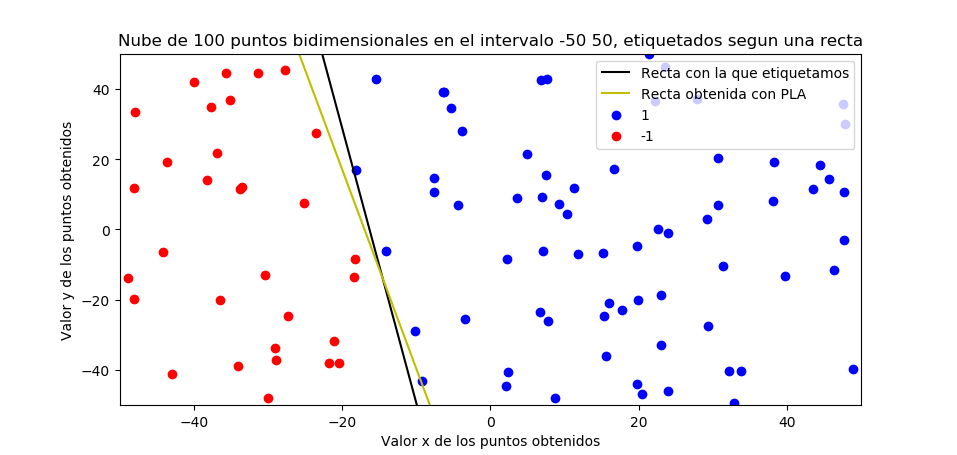
\includegraphics[scale = 0.70]{ej-2-PLA.png}
 		 \caption{Ejecución de PLA sobre una muestra uniforme etiquetada con una recta, sin ruido y $w = \{0, 0, 0\}$}
  		\label{fig:ej2-PLA}

\end{figure}

Vemos como consigue una recta en la que no etiqueta ningún punto de forma errónea, sin embargo es bastante distinta a la recta original. Esto se debe a que el número de puntos es bajo, para el algoritmo Perceptron es muy importante tener una muestra considerable de datos, ya que el ajuste se usa únicamente con los datos.

Como vemos en la salida, para este caso, el número medio de iteraciones necesarias para converger es el siguiente:

\begin{lstlisting}
W obtenida: [761.          44.78448243   7.88963959]
Iteraciones: 116
\end{lstlisting}

Ahora ejecutaremos otras diez veces el algoritmo, sin embargo, usaremos un vector de pesos inicial con valores aleatorios escogidos de forma uniforme entre [0, 1], con lo que ejecutando lo siguiente:

\begin{lstlisting}
iterations = []
for i in range(0,10):
	w_0 = simula_unif(3, 1, [0, 1]).reshape(1, -1)[0]
	w, iteraciones = ajusta_PLA(puntos_2d, etiquetas, np.Inf, w_0)
	iterations.append(iteraciones)
\end{lstlisting}

Obtenemos lo siguiente:

\begin{lstlisting}
Valor medio de iteraciones necesario para converger con 10 w_0 aleatorios entre [0, 1]: 82.1
\end{lstlisting}


Vemos como la diferencia de iteraciones es bastante significante, y esto es debido a que el vector inicial en el primer caso, al valer 0 todos sus componentes, es una recta sobre el eje x, lo que hace que necesite iteraciones extra ya que al inicializado de forma aleatoria solo necesitará corregir su inclinación y el punto en el eje x.


\subsubsection{Ejecución del algoritmo con ruido}

En este apartado se nos pide ejecutar la misma prueba, pero tras aplicar ruido de igual forma al ejercicio 1, apartado 2, sección b:

\begin{lstlisting}
w_0 = np.zeros(3)

w, iteraciones = ajusta_PLA(puntos_2d, etiquetas, 10000, w_0)
\end{lstlisting}

Más adelante explicaremos porque en este caso establecemos un límite de iteraciones.

\begin{figure}[H]
  \centering
      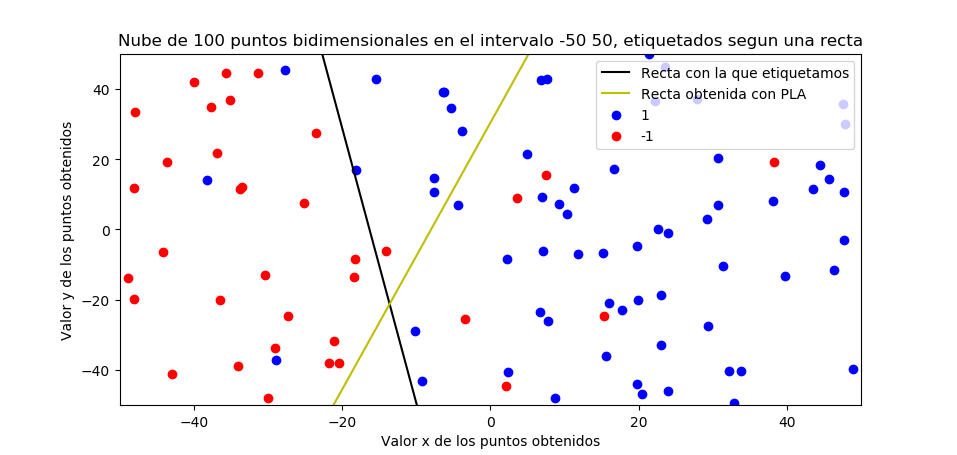
\includegraphics[scale = 0.70]{ej-2-PLA-ruido.png}
 		 \caption{Ejecución de PLA sobre una muestra uniforme etiquetada con una recta, con ruido y $w = \{0, 0, 0\}$}
  		\label{fig:ej2-PLA}

\end{figure}

En este caso obtenemos los siguientes resultados:

\begin{lstlisting}
W obtenida: [452.          56.54560859 -14.87894933]
Iteraciones: 10000
\end{lstlisting}

Vemos como en este caso utiliza todas las iteraciones y no conseguimos a obtener un óptimo que nos separe totalmente las etiquetas, ya que el ruido se lo impide. Al estar usando una recta, con dos puntos con ruido entra en bucle infinito, ya que el primer punto modifica el vector de pesos, dejando el segundo punto fuera y viceversa, es decir, el ruido hace que siempre encuentre mejora, ya que la recta no es capaz de separar los puntos con ruido. Esto veremos más adelante como solucionarlo usando el algoritmo Pocket, que añadirá memoria al algoritmo PLA, y permitirá trabajar con ruido, cosa que este algoritmo, como claramente vemos, no contempla.


Si ejecutamos la misma prueba diez veces pero con el vector de peso con valores iniciales aleatorios, obtenemos lo siguiente:

\begin{lstlisting}
Valor medio de iteraciones necesario para converger (no converge, es el máximo de iteraciones): 10000.0
\end{lstlisting}

Vemos como usa todas las iteraciones en las diez ejecuciones, y no llega a converger por culpa del ruido, como hemos comentado.


\subsubsection{Conclusiones}

Con este ejercicio hemos aprendido como funciona el algoritmo Perceptron, que aunque con ruido no es una buena opción, si sabemos que los datos son totalmente separables sabemos que encontrará una solución que los separe totalmente en tiempo finito, luego siempre es una buena opción si sabemos que en los datos no existe ruido.


\newpage

\subsection{Regresión Logística}

En este apartado implementaremos Regresión Logística con Gradiente Descendente Estocástico. Para representar el problema el conjunto de datos será una serie de 100 puntos escogidos aleatoriamente de forma uniforme en [0, 2] x [0, 2] y, como nos pide el ejercicio, serán etiquetados de acuerdo a una recta que pasará por dos puntos aleatorios del conjunto de datos.

\begin{lstlisting}
intervalo_trabajo = [0, 2]

x = simula_unif(100, 2, intervalo_trabajo)


# escogemos dos puntos y hacemos que la recta pase por estos
puntos_recta = np.random.choice(x.shape[0], 2, replace=False)

# ecuacio nde una recta: m = y_2 - y_1 / x_2 - x_1

a = (x[puntos_recta[1]][1] - x[puntos_recta[0]][1]) / (x[puntos_recta[1]][0] - x[puntos_recta[0]][0])

# y = ax + b

b = x[puntos_recta[0]][1] - (a*x[puntos_recta[0]][0])
\end{lstlisting}

\begin{figure}[H]
  \centering
      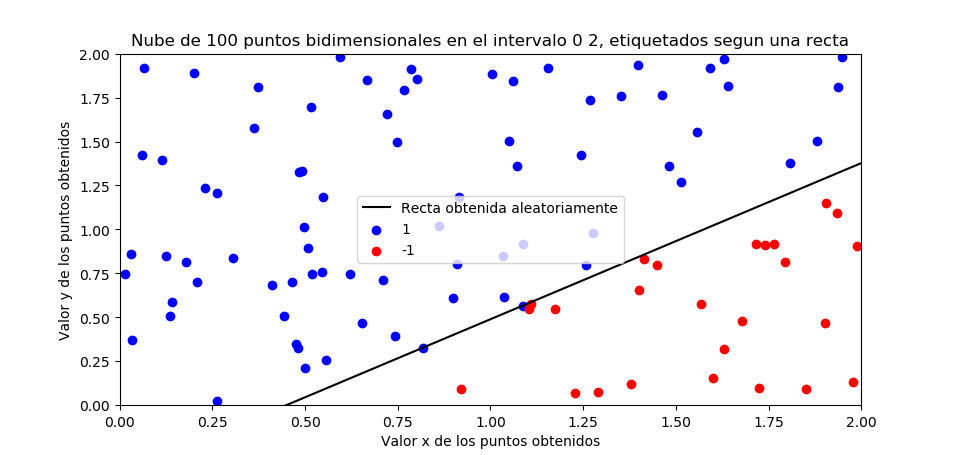
\includegraphics[scale = 0.70]{ej-2-puntos.png}
 		 \caption{Puntos seleccionados aleatoriamente y recta que pasa por dos de esos dos puntos}
  		\label{fig:ej2-puntos}

\end{figure}

\subsubsection{Implementación de Regresión Logística con SGD}

Para la implementación usaremos el algoritmo SGD usado en la práctica anterior además del criterio de aprendizaje ERM (Empirical Risk Minimization), que como vemos en las diapositivas de teoría podemos aplicar Regresión Logística:

\begin{lstlisting}
def error_erm(x, y, w):

	num_elementos = x.shape[1]

	error = np.float64(0.0)

	for i in range(num_elementos):
		error += np.log(1 + np.e**(-y[i]*w.T.dot(x[i])))

	error = error/num_elementos

	return error

def grad(x, y, w):

	return -(y * x)/(1 + np.exp(y * w.T.dot(x)))



def sgdRL(x, y, tasa_aprendizaje, error_permitido = 0.01):
    #
	# diapositiva 17, jussto antes del metodo de newton

	# el tamaño de w será dependiendo del numero de elementos de x
	w = np.zeros((x.shape[1],), np.float64)
	w_ant = w.copy()

	acabar = False

	epocas = 0


	# en este caso solo tenemos de condicion las iteraciones
	while not acabar:

		# aplicamos una permutacion aleatoria a los indices del minibatch
		indices_minibatch = np.random.choice(x.shape[0], x.shape[0], replace=False)

		# tamaños de minibatch = 1
		for i in indices_minibatch:
			w = w - tasa_aprendizaje * grad(x[i], y[i], w)

		epocas += 1
		dist = np.linalg.norm(w_ant - w)

		if dist < error_permitido:
			acabar = True

		w_ant = w.copy()


	return w, epocas
\end{lstlisting}

Como función de gradiente usamos la dada en el material para realizar la práctica, y como vemos, el tamaño de minibatch es de 1, como nos recomendaron al hacer la práctica.

La función de error es la vista en teoría para ERM, y vemos que nuestro algoritmo sigue los pasos dados por el ejercicio:

\begin{enumerate}
	\item Inicializar el vector de pesos a 0.
	\item Mientras la variación entre el vector de pesos actual y el vector de pesos de la siguiente época sea mayor al error permitido, ejecutar el algoritmo otra época.
	\item Aplicar una permutación aleatoria en el orden de los datos antes de cada época.
\end{enumerate}

Con esto, ejecutamos el algoritmo de la siguiente forma, con 0.01 de $\eta$ y 0.01 de error:

\begin{lstlisting}
x = np.c_[np.ones((x.shape[0], 1), dtype=np.float64), x]

w, epocas = sgdRL(x, etiquetas, 0.01, 0.01)
\end{lstlisting}

Con el que obtenemos el siguiente ajuste:

\begin{figure}[H]
  \centering
      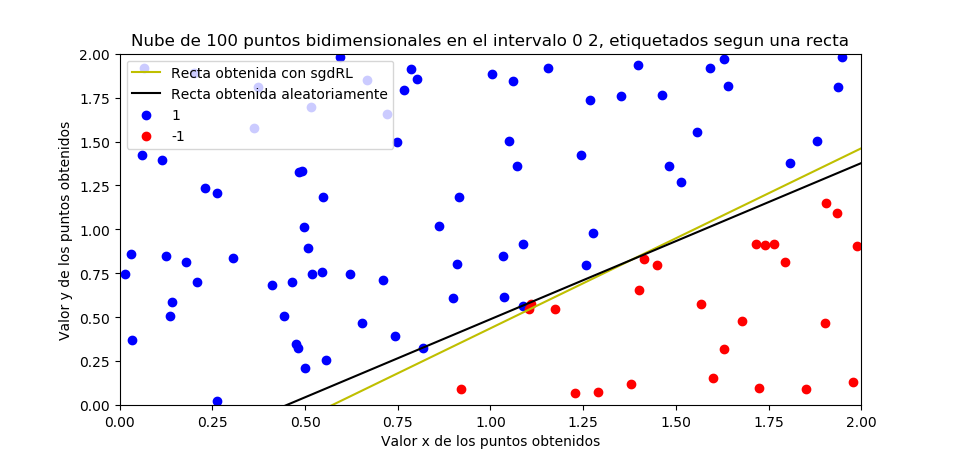
\includegraphics[scale = 0.70]{ej-2-SGR-RL.png}
 		 \caption{Ajuste obtenido con Regresión Logística con SGD}
  		\label{fig:ej2-SGR-RL}

\end{figure}

\begin{lstlisting}
W obtenida: [ 3.45912615 -6.01951788  5.87111196]
 Épocas: 10000
Error obtenido dentro de la muestra (Ein): 0.013165327735081708
\end{lstlisting}

Vemos como el ajuste es bastante bueno, con un error de 0.013, ahora veremos el error en $E_{out}$ con una muestra generada de la misma forma, pero con 1000 puntos en lugar de 100:

\begin{figure}[H]
  \centering
      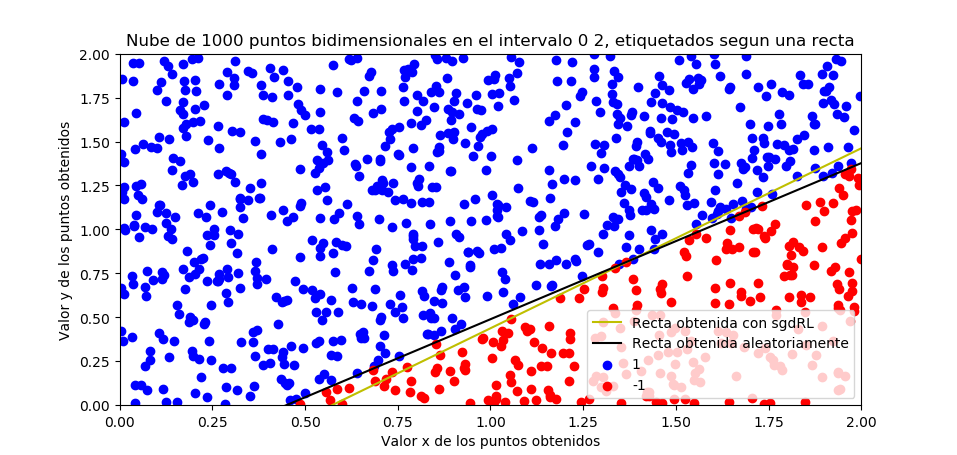
\includegraphics[scale = 0.70]{ej-2-SGR-RL-1000.png}
 		 \caption{Ajuste obtenido con Regresión Logística con SGD en $E_{out}$ con 1000 puntos}
  		\label{fig:ej2-SGR-RL}

\end{figure}

En el que obtenemos el siguiente error:

\begin{lstlisting}
Error obtenido fuera de la muestra (Eout): 0.07828587637844557
\end{lstlisting}

Vemos como el error es mayor, pero sigue siendo bastante más bajo.



\section{Ejercicio bonus: Clasificación de Dígitos}

Para este ejercicio volvemos a usar los datos de intensidad promedio y de simetría en clasificación de números, pero en lugar de clasificar los números 1 y 5 usaremos los datos de los números 4 y 8.

\subsection{Planteamiento del problema}

En nuestro caso, queremos clasificar un conjunto de números escritos a manos. En concreto, para que el problema sea binario clasificaremos dos números, el 4 y el 8, en los que intentaremos aprender una función  $g$.

Para esto usaremos un conjunto de entrenamiento y otro conjunto de test e intentaremos conseguir un ajuste usando modelos de Regresión Lineal y aplicando el algoritmo PLA-Pocket como mejora, viendo como esto puede ser una mejora sustancial para métodos que se comportaban bien, sin embargo esto hará que se comporten aún mejor ya que como veremos existe mucho más ruido, lo que dificulta el hacer un buen ajuste como hemos visto.


\begin{figure}[H]
  \centering
      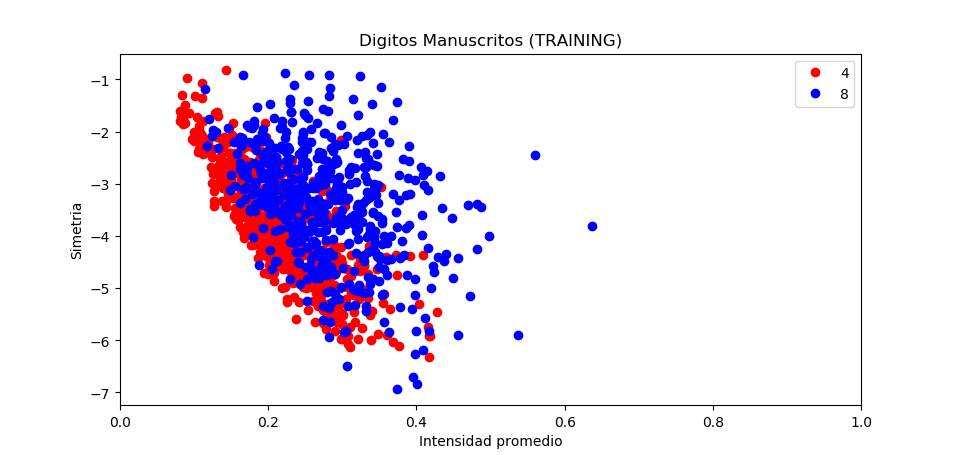
\includegraphics[scale = 0.70]{datos_bonus.png}
 		 \caption{Datos de los dígitos 4 y 8 (conjunto de entrenamiento)}
  		\label{fig:bonus_entrenamiento}

\end{figure}

\begin{figure}[H]
  \centering
      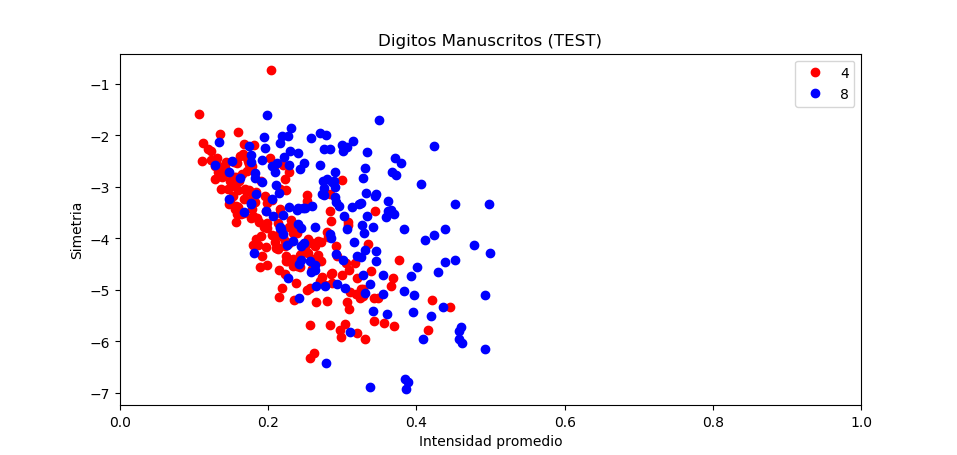
\includegraphics[scale = 0.70]{datos_bonus_test.png}
 		 \caption{Datos de los dígitos 4 y 8 (conjunto de test)}
  		\label{fig:bonus_test}

\end{figure}

\subsection{Implementación del problema usando SGD}

Para resolver este problema, primero tenemos que implementar el Gradiente Descendente Estocástico, ya que será el modelo de Regresión Lineal que usaremos. El algoritmo será el mismo que en la práctica anterior, pero con una pequeña modificación, ya que en la práctica anterior implemente una versión distinta al SGD vista en teoría y dicha versión no comprobaba que aprenda al menos una vez de cada dato, mientras que esta versión si:

\begin{lstlisting}
# Funcion para calcular el error
def Err(x,y,w):
	## Función dada en las diapositivas:
	#
	# E_in(w) = 1/N * SUM(w^T * x_n - y_n)^2
	#
	# basicamente, hacemos w * x - y al cuadrado, y le hacemos la media

	# https://docs.scipy.org/doc/numpy/reference/generated/numpy.square.html
	# cambiamos la forma de y, ya que como vemos en las diapositivas, y tiene una columna
	# y muchas filas, pero aqui tenemos una fila y muchas columnas
	err = np.square(x.dot(w) - y.reshape(-1,1))

	# https://docs.scipy.org/doc/numpy/reference/generated/numpy.mean.html
	err.mean()

	return err

def dErr(x, y, w):
	#derivada como hemos visto en teoria
	# la parte interna sigue igual
	derivada = x.dot(w) - y.reshape(-1,1)

	# el cuadrado pasa a ser un *2, y restamos una al exponente
	derivada = 2 * np.mean(x * derivada, axis=0)

	derivada = derivada.reshape(-1, 1)

	return derivada


def sgd(x, y, tasa_aprendizaje, tam_batch, maxIteraciones = 4000):
    #
	# diapositiva 17, jussto antes del metodo de newton

	# el tamaño de w será dependiendo del numero de elementos de x
	w = np.zeros((x.shape[1], 1), np.float64)

	iterations = 0

	nueva_epoca = False
	indice_actual = 0

	indices_minibatch = np.random.choice(x.shape[0], x.shape[0], replace=False)

	# en este caso solo tenemos de condicion las iteraciones
	while iterations < maxIteraciones:

		iterations = iterations + 1

		if nueva_epoca:
			nueva_epoca = False
			indices_minibatch = np.random.choice(x.shape[0], x.shape[0], replace=False)

		if indice_actual+tam_batch < x.shape[0]:
			minibatch = indices_minibatch[indice_actual:indice_actual+tam_batch]
			indice_actual += tam_batch
		else:
			minibatch = indices_minibatch[indice_actual:x.shape[0]]
			indice_actual = 0
			nueva_epoca = True


		w = w - tasa_aprendizaje * dErr(x[minibatch], y[minibatch], w)
		iterations += 1



	return w, iterations
\end{lstlisting}

Vemos como en este algoritmo, ya si se tiene en cuenta que se aprenda de todos los elementos al menos una vez, aunque se recorren de forma aleatoria.

\subsubsection{Ejecución del algoritmo}

Este algoritmo nos da el siguiente ajuste en $E_{in}$:

\begin{figure}[H]
  \centering
      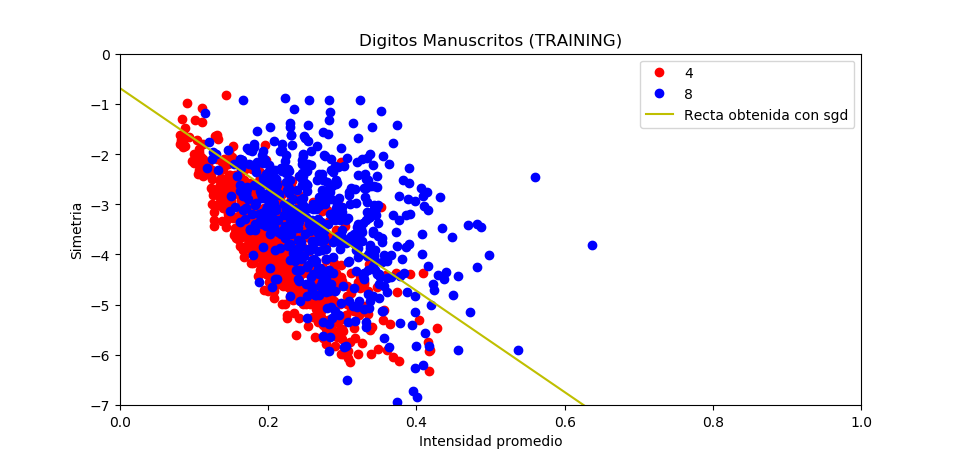
\includegraphics[scale = 0.70]{bonus_sgd.png}
 		 \caption{Ajuste obtenido con SGD en $E_{in}$}
  		\label{fig:ej2-SGR-RL}

\end{figure}

Lo cual nos da el siguiente error:

\begin{lstlisting}
Error obtenido usando sgd dentro de la muestra (Ein):  0.7694165537758165
\end{lstlisting}


Y el siguiente ajuste en $E_{test}$:

\begin{figure}[H]
  \centering
      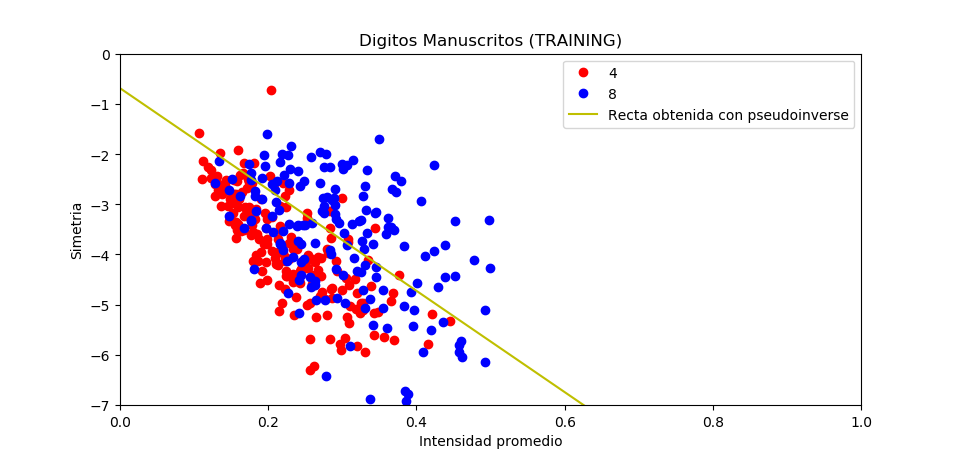
\includegraphics[scale = 0.70]{bonus_sgd-test.png}
 		 \caption{Ajuste obtenido con SGD en $E_{test}$}
  		\label{fig:ej2-SGR-RL}

\end{figure}

Lo cual nos da el siguiente error:

\begin{lstlisting}
Error obtenido usando sgd para los datos de test (Etest):  0.8175413200852162
\end{lstlisting}

Vemos como el error es bastante alto debido al ruido que presentan los datos. Intentaremos mejorar el ajuste aplicando el algoritmo PLA-Pocket que explicaré a continuación.

\newpage

\subsection{Implementación del algoritmo usando PLA-Pocket}

El algoritmo se basa en ejecutar el algoritmo Perceptron, implementado y usado en el segundo ejercicio de esta práctica, pero almacenando el mejor valor que ha tenido hasta el momento, ya que como sabemos el algoritmo Perceptron no tiene ningún tipo de memoria. por lo que no almacena datos sobre iteraciones anteriores.


\begin{lstlisting}
def signo(x):
	if x >= 0:
		return 1
	return -1


def num_errores_puntos(x, y, w):

	errores = 0
	for i in range(len(x)):
		if signo(w.T.dot(x[i])) != y[i]:
			errores += 1

	errores = errores/len(x)

	return errores

def simula_unif(N, dim, rango):
	return np.random.uniform(rango[0],rango[1],(N,dim))


def ajusta_PLA(datos, label, max_iter, vini):
    #CODIGO DEL ESTUDIANTE
	w = np.copy(vini)
	mejora = True
	iteraciones = 0

	while mejora and iteraciones < max_iter:
		mejora = False

		for i in range(0, len(datos)):
			valor = signo(w.T.dot(datos[i]))

			if valor != label[i]:
				w = w + label[i] * datos[i].reshape(-1, 1)
				mejora = True

		iteraciones += 1

	return w, iteraciones


#POCKET ALGORITHM
def pocket(x, y, iteraciones, w_ini):

	# en el ej 2 nos daba mejores resultados si el comienzo lo haciamos aleatorio entre [0, 1]
	#w_mejor = simula_unif(3, 1, [0, 1]).reshape(1, -1)[0]
	w_mejor = w_ini.copy()

	ein_w_mejor = num_errores_puntos(x, y, w_mejor)
	w = w_mejor.copy()

	it = 0

	while it < iteraciones:
		w, basura = ajusta_PLA(x, y, 1, w.copy())
		ein_w = num_errores_puntos(x, y, w)
		if ein_w < ein_w_mejor:
			w_mejor = w.copy()
			ein_w_mejor = ein_w

		it += 1

	return w_mejor
\end{lstlisting}


Vemos como en este caso la función de error usada es un conteo de los puntos que están mal clasificados.

Básicamente, ejecutamos el PLA (algoritmo Perceptron) tantas veces como iteraciones llamemos al algoritmo PLA-Pocket, he decidido que la llamada al algoritmo PLA sea de únicamente una época, ya que como hemos comentado, el principal problema del PLA es que no tiene memoria, por lo que si ejecutamos con más de una época es posible que se salte el mínimo que estamos buscando.

Como nos pide el ejercicio, el vector de pesos inicial para el algoritmo Pocket será el ajuste obtenido por el algoritmo SGD, de forma que intentaremos mejorar el ajuste obtenido por SGD.

Obtenemos los siguientes resultados:

\begin{figure}[H]
  \centering
      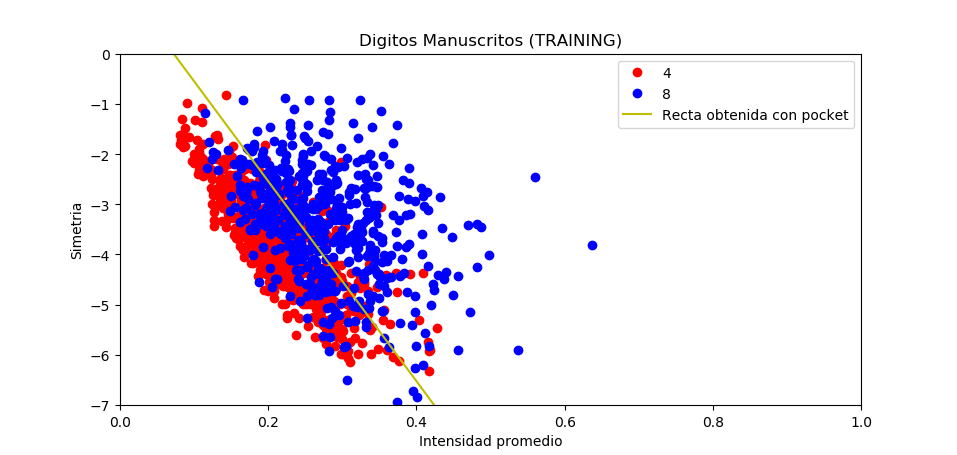
\includegraphics[scale = 0.70]{bonus_pocket.png}
 		 \caption{Ajuste obtenido con PLA-Pocket en $E_{in}$}
  		\label{fig:bonus-pla-pocket}

\end{figure}

\begin{lstlisting}
Error obtenido usando pocket dentro de la muestra (Ein):  0.22445561139028475
\end{lstlisting}

\begin{figure}[H]
  \centering
      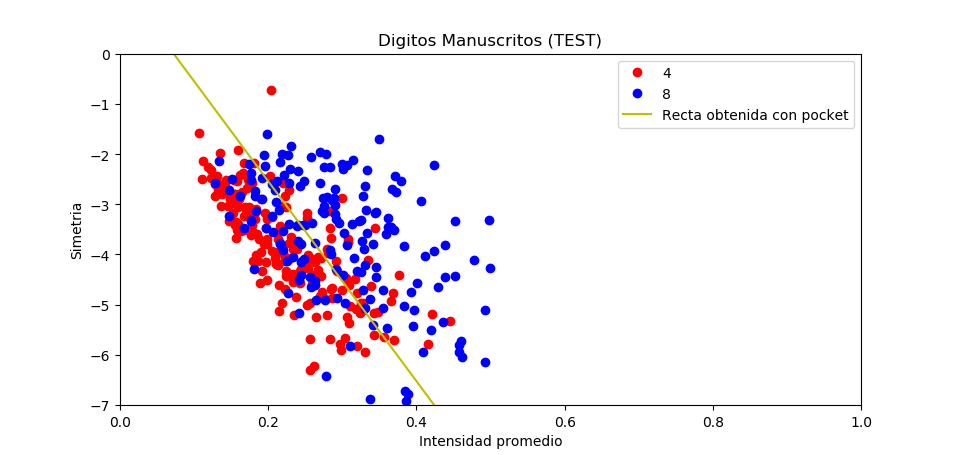
\includegraphics[scale = 0.70]{bonus_pocket-test.png}
 		 \caption{Ajuste obtenido con PLA-Pocket en $E_{test}$}
  		\label{fig:bonus-pla-pocket}

\end{figure}


\begin{lstlisting}
Error obtenido usando pocket para los datos de test (Etest):  0.2568306010928962
\end{lstlisting}


Vemos como hemos reducido en gran cantidad el error, y el error obtenido es principalmente por el ruido.


\subsection{Calculo de la cota del error fuera de la muestra}

Vamos a calcular una cota sobre el verdadero valor de $E_{out}$. Para esto usaremos lo aprendido en teoría:

$$ E_{out}(h) \leq E_{in}(h) + \sqrt{\frac{1}{2*N}*log\frac{2}{\delta}} $$

Podemos calcular dos cotas del error, usando $E_{in}$ o usando $E_{out}$. Como se nos pide en el ejercicio, usaremos $\delta = 0,05$

\subsubsection{Calculo de la cota usando el error en la muestra}

$$ E_{out}(h) \leq E_{in}(h) + \sqrt{\frac{1}{2*N}*log\frac{2}{\delta}} $$

Obtenemos la siguiente cota:

\begin{lstlisting}
Cota de Eout usando Ein:  0.26375900679491193
\end{lstlisting}



\subsubsection{Calculo de la cota usando el error en el test}

$$ E_{out}(h) \leq E_{test}(h) + \sqrt{\frac{1}{2*N}*log\frac{2}{\delta}} $$

Obtenemos la siguiente cota:

\begin{lstlisting}
Cota de Eout usando Ein:  0.29613399649752337
\end{lstlisting}

Vemos como al calcular las cotas, la cota en $E_{test}$ es mayor ya que el segundo sumando es el mismo para ambas cotas, sin embargo $E_{test}$ es mayor.

\newpage

\section{Referencias, material y documentación usada}


\begin{thebibliography}{9}

\bibitem{teoria}
Diapositivas de teoría

\bibitem{documentacion-numpy}
Documentación de NumPy:

\url{https://docs.scipy.org/doc/numpy-1.15.0/reference/generated/numpy.random.choice.html}

\url{https://docs.scipy.org/doc/numpy/reference/generated/numpy.transpose.html}

\url{https://docs.scipy.org/doc/numpy/reference/generated/numpy.dot.html}

\url{https://docs.scipy.org/doc/numpy/reference/generated/numpy.linalg.inv.html}

\url{https://docs.scipy.org/doc/numpy/reference/generated/numpy.c_.html}

\url{https://docs.scipy.org/doc/numpy/reference/generated/numpy.square.html}

\url{https://docs.scipy.org/doc/numpy/reference/generated/numpy.mean.html}


\end{thebibliography}

\end{document}
